\documentclass[a4 paper]{article}

\usepackage{amsmath, amsthm, amsfonts} 
\usepackage[skip = 10pt, indent = 30pt]{parskip}    
\usepackage{setspace}
\onehalfspacing
\usepackage{caption}
\usepackage{subcaption}
\usepackage{pdfpages}\usepackage{booktabs}
\usepackage{textcomp}
\usepackage{amssymb}
\usepackage[document]{ragged2e}
\usepackage{bm}
\usepackage[brazil]{babel}



\newcommand{\parag}{\hspace{30pt}}


\title{TAC - Seizure Recognition}
\author{Yuri Shumyatsky - 231012826\\Gabriel Gonçalves Caldo - 231034627\\Pedro Araujo Cordeiro Viana - 202067452}
\date{\today}
\begin{document}

\maketitle
\newpage

\section{Introdução}


\section{MutRoSe - iHTN's}
\parag Dada a escolha da missão como sendo a Seizure Recognition do repositório RoboMax, foi utilizado a extensão do VSCode para o uso do MutRoSe e para a decomposição da missão e elaboração das iHTN's. 

\begin{table}[h]
\centering
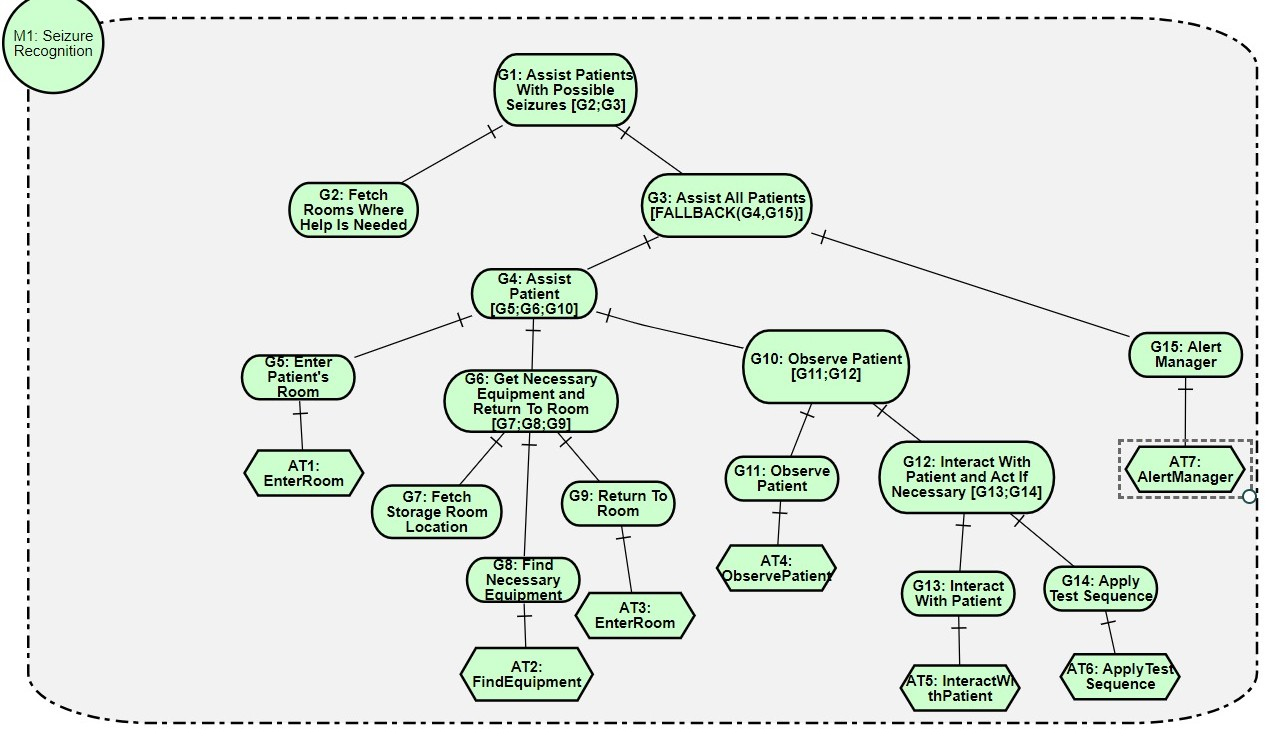
\includegraphics[scale=0.3]{figuras/gm}
\end{table}
\begin{center}
Figura 1: Goal Model da Missão
\end{center}
\vspace{15pt}

Ao decompor essa missão, foram geradas inúmeras iHTNs (em torno de 1340), mas foi selecionada a iHTN de número $666$ para basear a construção da Behavior Tree.
\vspace{15pt}\vspace{15pt}

\begin{table}[h]
\centering
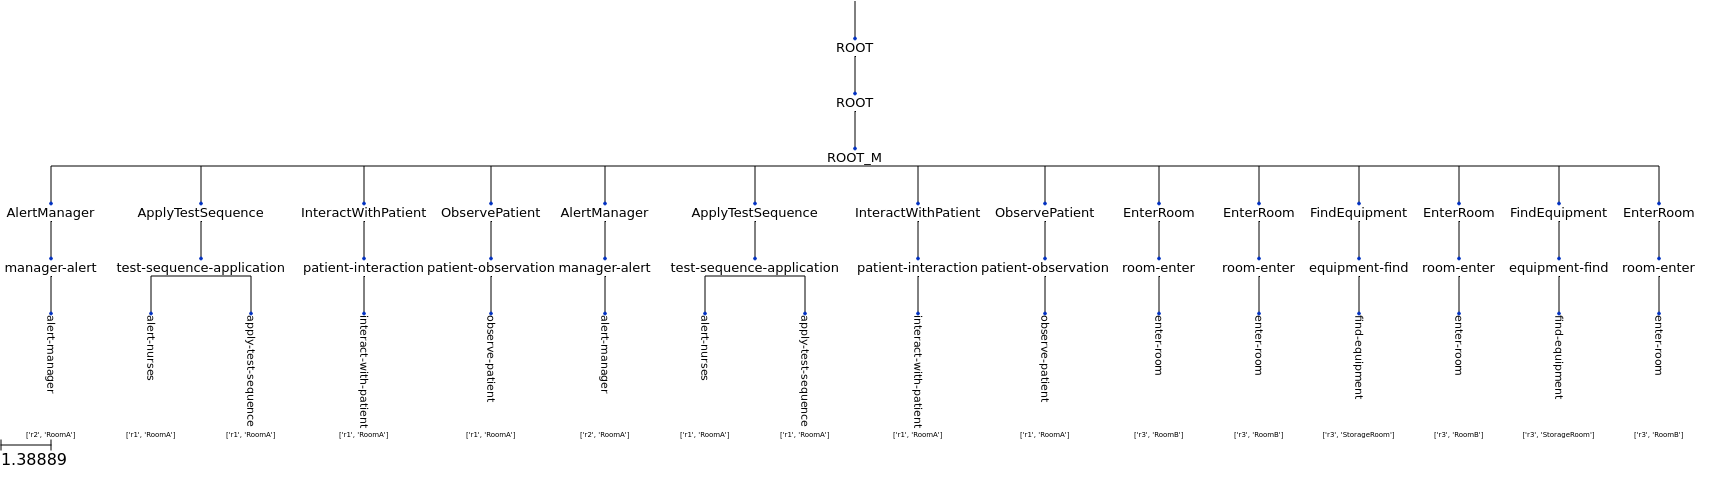
\includegraphics[scale=0.25]{figuras/ihtn_666}
\end{table}
\begin{center}
Figura 2: iHTN 666
\end{center}
\vspace{30pt}

O resultado é portanto a Behavior Tree da Figura 3.

\newpage
\begin{table}[h]
\centering
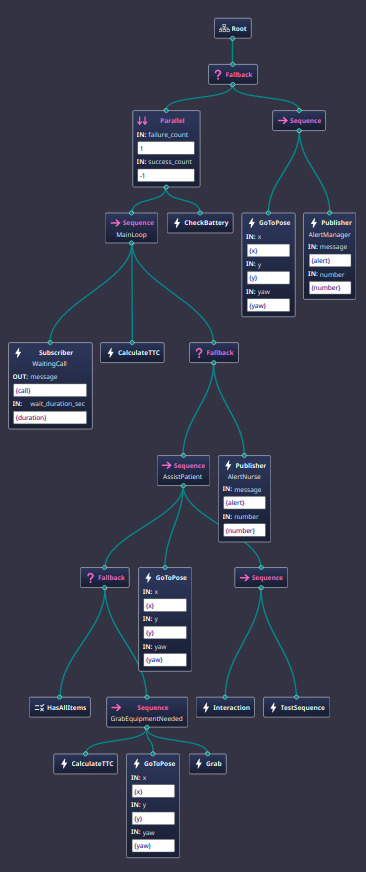
\includegraphics[scale=0.5]{figuras/bt}
\end{table}
\begin{center}
Figura 3: BT simulada no Groot
\end{center}

\section{Configuração do Mapa}
\parag Apesar dos arquivos para o mapa do hospital terem sido providenciados, foram gastas múltiplas horas tentando fazer com que a simulação usasse os arquivos corretos, mas não houve sucesso. 

De fato,  o mais próximo alcançado foi a presença apenas das paredes, sem texturas ou objetos, como mostra a Figura 4.

%Figura 4

Além disso, foi testado também com o mapa do CiC, mas não houve sucesso.


\begin{table}[h]
\centering
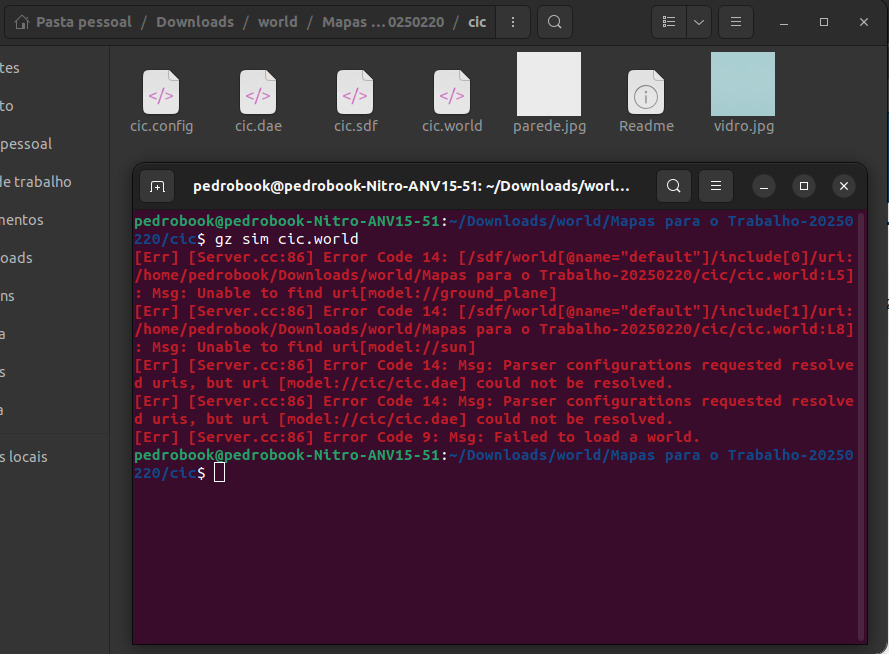
\includegraphics[scale=0.4]{figuras/cicerror}
\end{table}
\begin{center}
Figura 5: Erro ao usar o mapa CiC
\end{center}

\section{Build}
\parag Ao tentar usar o CMake para organizar os arquivos e construir um binário, ocorreram erros que impediram a execução da Behavior Tree. 

Principalmente, um erro foi o não reconhecimento dos ports do nó de controle "Paralelo", apesar do nó ser o padrão do programa Groot 2. 




\section{Conclusão}
\end{document}
